\documentclass[11pt]{article}

\usepackage[margin=1in]{geometry}
\usepackage[T1]{fontenc}
\usepackage{lmodern}
\usepackage{amsmath,amssymb}
\usepackage{booktabs}
\usepackage{tabularx}
\usepackage{longtable}
\usepackage{enumitem}
\usepackage{xcolor}
\usepackage{tikz}
\usepackage[hidelinks]{hyperref}
\usetikzlibrary{arrows.meta,fit,positioning,shapes.geometric}

\definecolor{Forest}{HTML}{153C32}
\definecolor{Mint}{HTML}{C9F0DC}
\definecolor{Cream}{HTML}{F8F6EF}
\definecolor{Rust}{HTML}{B65738}
\definecolor{Muted}{HTML}{64706C}

\hypersetup{colorlinks=true,linkcolor=Forest,urlcolor=Rust}
\setlist[itemize]{leftmargin=1.5em,itemsep=0.25em}
\setlist[enumerate]{leftmargin=1.7em,itemsep=0.35em}
\renewcommand{\arraystretch}{1.2}

\title{Student Evidence and Tutoring Interaction Notes}
\author{Digital Professor Prototype}
\date{September 2026}

\begin{document}
\maketitle
\tableofcontents
\section{Purpose and scope}

This note defines an interaction and integration layer for a Digital Professor. The layer connects LLM-assisted syllabus reading, lecture-note CAG/RAG, multimodal student input, tutoring decisions, and chat or animated-avatar delivery. Its central contract is structured \emph{Student Evidence}: a traceable representation of what the student submitted, how the system interpreted it, and what happened after an intervention.

The design is an interaction contract rather than a final architecture. It separates three responsibilities:

\begin{itemize}
    \item The \textbf{interaction and integration layer} coordinates course setup, context retrieval, multimodal interaction, evidence construction, and response delivery.
    \item The \textbf{Student Evidence service} captures what the student actually submitted, confirms ambiguous recognition, and produces the canonical interaction record.
    \item The \textbf{system state and decision layer} updates its estimate of the student's current understanding and selects the next pedagogical action.
    \item The \textbf{presentation layer} renders that action in the chat, equation renderer, sketchpad, document viewer, or another appropriate interface.
\end{itemize}

The attached tutoring flows provide two complementary patterns. The first develops a proof of sufficiency for
\[
X_i \overset{\mathrm{iid}}{\sim} \operatorname{Unif}(0,\theta),
\qquad T(X)=\max(X_1,\ldots,X_n),
\]
including initial elicitation, targeted hints, misconception handling, a comprehension check, and transfer problems. The corrected second flow diagnoses why substitution does not fit $\int x\cos x\,dx$, elicits another integration method, lets the student repair their own work, and ends with similar and contrasting examples.

\section{Integrated system role}

The project combines four capabilities that otherwise operate on different representations and timescales. The interaction and integration layer provides the shared identifiers, events, provenance, and handoffs that allow them to behave as one tutoring system.

\noindent\begin{tabularx}{\textwidth}{@{}p{0.24\textwidth}p{0.29\textwidth}X@{}}
\toprule
\textbf{Capability} & \textbf{Produces or consumes} & \textbf{Integration responsibility} \\
\midrule
LLM-assisted syllabus reading & Course identity, overview, policies, schedule, assessments, learning outcomes, and extraction confidence & Build a versioned course profile, preserve the syllabus source locations, and expose uncertainty or missing fields instead of inventing them. \\
Lecture-note CAG/RAG & Indexed notes, retrieved passages, page IDs, retrieval scores, and citations & Request context for the current student turn, keep retrieved material separate from student evidence, and permit citations only to supplied passages. \\
Multimodal interaction & Text, speech, images, handwriting, equations, files, recognition candidates, and confirmations & Convert every modality into a common submission envelope while preserving the original artifact and modality-specific provenance. \\
Digital animated avatar & Spoken and visual presentation, real-time turn events, interruption state, and delivery acknowledgements & Convert an approved pedagogical action into a delivery package, synchronize text and speech, and record what was actually presented to the student. \\
Student Evidence and decisions & Confirmed evidence, learner-state updates, chosen actions, revisions, and reassessment results & Maintain the shared interaction timeline that connects course context, student behavior, system action, and outcome. \\
\bottomrule
\end{tabularx}

\subsection{Integration architecture}

\begin{center}
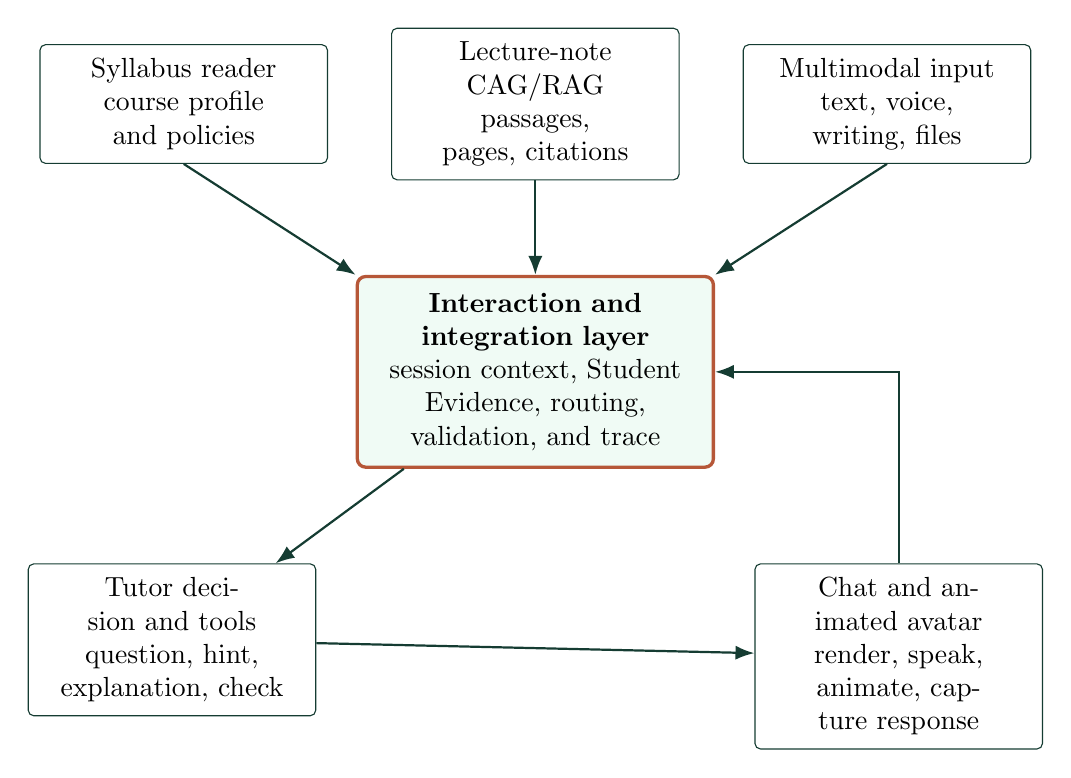
\begin{tikzpicture}[
  node distance=7mm and 8mm,
  source/.style={draw=Forest,rounded corners=2pt,fill=white,align=center,
    text width=3.3cm,minimum height=1.05cm,inner sep=5pt},
  core/.style={draw=Rust,very thick,rounded corners=3pt,fill=Mint!28,align=center,
    text width=4.1cm,minimum height=1.35cm,inner sep=6pt},
  arrow/.style={-{Latex[length=2.4mm]},thick,draw=Forest}
]
\node[source] (syllabus) {Syllabus reader\\course profile and policies};
\node[source,right=of syllabus] (notes) {Lecture-note CAG/RAG\\passages, pages, citations};
\node[source,right=of notes] (multi) {Multimodal input\\text, voice, writing, files};
\node[core,below=12mm of notes] (integration) {\textbf{Interaction and integration layer}\\session context, Student Evidence, routing, validation, and trace};
\node[source,below left=12mm and 5mm of integration] (decision) {Tutor decision and tools\\question, hint, explanation, check};
\node[source,below right=12mm and 5mm of integration] (delivery) {Chat and animated avatar\\render, speak, animate, capture response};
\draw[arrow] (syllabus.south)--(integration.north west);
\draw[arrow] (notes)--(integration);
\draw[arrow] (multi.south)--(integration.north east);
\draw[arrow] (integration)--(decision);
\draw[arrow] (decision)--(delivery);
\draw[arrow] (delivery.north)|-(integration.east);
\end{tikzpicture}
\end{center}

The integration layer is responsible for orchestration and traceability, not for replacing each subsystem. The syllabus reader remains responsible for extraction, CAG/RAG for retrieval, recognition providers for modality conversion, the tutor policy for pedagogical choice, and the avatar engine for animation. Their outputs cross a validated contract before affecting another component.

\section{Student Evidence module contract}

Within the broader interaction and integration layer, the Student Evidence module is the shared contract between student-facing interaction, recognition, course context, learner state, tutoring decisions, avatar delivery, and evaluation. Its central responsibility is to create a trustworthy record of \emph{what the student provided, how it was interpreted, and what interaction produced it}. Central does not mean that it performs every task itself.

\subsection{Component boundary}

The module \textbf{owns} submission identity, evidence-event construction, ambiguity status, confirmation history, attempt and revision links, schema validation, provenance, and publication of validated evidence. It may coordinate recognition and parsing tools, but it does not own their internal models.

The module does \textbf{not} decide mastery, choose the next tutoring strategy, generate the student-facing explanation, perform OCR by itself, or silently correct mathematical work. Those responsibilities remain with the learner-state, decision, presentation, and recognition components. This boundary keeps the central evidence record stable when one provider or tutoring policy changes.

\subsection{Inputs}

\noindent\begin{tabularx}{\textwidth}{@{}p{0.22\textwidth}p{0.30\textwidth}X@{}}
\toprule
\textbf{Input} & \textbf{Required contents} & \textbf{Source and purpose} \\
\midrule
Submission envelope & Submission ID, session and turn IDs, timestamp, modality manifest, raw artifact reference, and student-entered text & Sent by the interface whenever the student asks a question, submits work, explains reasoning, confirms recognition, or revises an answer. \\
Interaction context & Current problem, course and concept identifiers, requested help level, and applicable assignment policy & Sent by the session controller so the same input can be interpreted in the correct learning context. \\
Eliciting action & Action ID, action type, pedagogical goal, and expected response type & Sent by the decision or action layer; identifies the question, hint, explanation, retry, or transfer task that prompted the response. \\
Recognition result & Candidate transcription, normalized text or mathematics, uncertain regions, alternatives, confidence, and provider metadata & Returned by handwriting, speech, OCR, or mathematical parsing tools. \\
Confirmation event & Candidate shown, student's confirmation or edit, time, and correction effort & Sent by the interface when a meaning-changing ambiguity requires student review. \\
Course context references & Retrieved passage IDs, document and page IDs, and retrieval provenance & Sent by the course-grounding component when the student's response refers to course material. \\
Module policy & Required fields, ambiguity thresholds, retention rules, tool permissions, privacy settings, and schema version & Supplied by system configuration so behavior is explicit and reproducible. \\
\bottomrule
\end{tabularx}

The module may accept missing optional context, but it must never invent a required identifier or treat absent recognition confidence as high confidence. Missing information produces an explicit status or restricted evidence event.

\subsection{Outputs}

\noindent\begin{tabularx}{\textwidth}{@{}p{0.24\textwidth}p{0.31\textwidth}X@{}}
\toprule
\textbf{Output} & \textbf{Contents} & \textbf{Consumer} \\
\midrule
Validated Student Evidence event & Confirmed or explicitly unresolved content, response type, claims and steps, uncertainty, context, links, evaluation status, and provenance & Learner-state updater, decision layer, evaluation pipeline, and audit log. \\
Confirmation request & Original region, rendered candidate, alternatives, reason for confirmation, and permitted response controls & Presentation layer, which asks the student a narrow clarification question. \\
Processing status & Received, recognizing, needs confirmation, evidence ready, partially resolved, or failed, with a reason code & Interface and session controller, so failures and waits are visible. \\
Evidence-ready notification & Evidence ID, session and turn IDs, schema version, and event location & Learner-state and decision components; prevents them from acting on incomplete input. \\
Audit and measurement record & Provider/model, settings, latency, token and cost data, confidence, corrections, and validation results & Evaluation, monitoring, and later model comparison. \\
Validation error & Missing field, invalid relationship, unsupported modality, tool failure, or policy violation with recoverable next step & Session controller and, when necessary, human-review queue. \\
\bottomrule
\end{tabularx}

Only a validated event or an explicitly labeled partially resolved event may leave the module as Student Evidence. Raw recognition output is never published as confirmed student work.

\subsection{Expected behaviors}

\begin{itemize}
    \item \textbf{Faithful capture:} preserve the raw submission and represent the student's content without correcting its mathematics or changing its meaning.
    \item \textbf{Modality independence:} produce the same core event structure for text, handwriting, speech, images, equations, and mixed input while retaining modality-specific details.
    \item \textbf{Confirmation before interpretation:} pause evidence finalization when a plausible alternative changes mathematical meaning.
    \item \textbf{Clear attribution:} distinguish student-authored content, recognition output, system interpretation, retrieved course content, and tool output.
    \item \textbf{Traceable revisions:} create a new event for a retry or revision and link it to the earlier attempt and intervention rather than overwriting history.
    \item \textbf{Safe failure:} return a visible, recoverable status when recognition, context retrieval, or validation fails. Do not fill gaps with guesses.
    \item \textbf{Idempotent processing:} receiving the same submission ID twice must not create two independent evidence events.
    \item \textbf{Versioned validation:} validate every event against a named schema and policy version before publication.
    \item \textbf{Minimum necessary data:} expose only the fields required by each consumer and enforce the configured retention and privacy rules.
    \item \textbf{Observable operation:} record enough provenance, latency, correction effort, and failure detail to evaluate the module later.
    \item \textbf{Cross-channel consistency:} deliver the same approved mathematical and pedagogical content in chat, speech, and avatar animation.
    \item \textbf{Grounded course use:} distinguish syllabus-derived course structure from lecture-note passages and cite only retrieved material.
    \item \textbf{Graceful degradation:} continue through text chat if an avatar, speech, recognition, or retrieval provider is unavailable, while recording the failure.
\end{itemize}

\subsection{Main functions}

The names below describe logical functions for future implementation; they do not require a particular language, API style, or deployment architecture.

\noindent\begin{tabularx}{\textwidth}{@{}p{0.27\textwidth}p{0.29\textwidth}X@{}}
\toprule
\textbf{Function} & \textbf{Responsibility} & \textbf{Result} \\
\midrule
\texttt{receive\_submission} & Validate IDs, modality, file references, and basic policy limits; persist the immutable envelope. & Accepted submission or actionable validation error. \\
\texttt{route\_recognition} & Select only an allowed recognizer or parser for each artifact and attach the minimum necessary context. & One or more recognition results with provenance. \\
\texttt{assess\_ambiguity} & Identify alternatives whose difference could change interpretation, correctness, or the next tutoring action. & Continue automatically or create a confirmation request. \\
\texttt{apply\_confirmation} & Record the student's confirmation or correction without deleting the original candidate. & Confirmed content and a traceable confirmation event. \\
\texttt{extract\_evidence} & Separate the problem, claims, equations, steps, answer, explanation, uncertainty, and response type. & Draft Student Evidence event with attributed fields. \\
\texttt{link\_interaction} & Attach the eliciting action, attempt, prior evidence, revision, course context, and source references. & Connected evidence event within the tutoring trajectory. \\
\texttt{validate\_evidence} & Check schema, required relationships, attribution, ambiguity status, and provenance. & Validated, partially resolved, or rejected event with reasons. \\
\texttt{publish\_evidence} & Store the validated event and notify authorized downstream consumers once. & Stable evidence ID and evidence-ready notification. \\
\texttt{export\_trace} & Assemble submissions, confirmations, evidence, actions, state changes, tools, and metrics in time order. & Reproducible trajectory for review and evaluation. \\
\bottomrule
\end{tabularx}

The surrounding integration layer adds four orchestration functions:

\begin{itemize}
    \item \texttt{initialize\_course\_workspace}: turn verified syllabus extraction into a versioned course profile and connect lecture-note indexes.
    \item \texttt{request\_course\_context}: retrieve relevant lecture passages and page references for the current evidence event and tutoring goal.
    \item \texttt{prepare\_delivery}: convert an approved tutoring action into channel-neutral text, mathematics, speech, and avatar cues without changing its meaning.
    \item \texttt{record\_delivery}: store what chat, speech, or the avatar actually presented, including interruptions, failures, and timing.
\end{itemize}

\subsection{Interfaces with the rest of the system}

\begin{itemize}
    \item The \textbf{student interface} sends submission and confirmation events and receives status or confirmation requests.
    \item The \textbf{recognition services} receive bounded artifacts and return candidates, alternatives, confidence, and provenance.
    \item The \textbf{syllabus-reading component} supplies a versioned course profile with field-level confidence and source locations.
    \item The \textbf{lecture-note CAG/RAG component} supplies verified passages and page references; document text cannot change module policy.
    \item The \textbf{learner-state component} receives validated evidence and returns a separate, provisional state update. It cannot rewrite the evidence event.
    \item The \textbf{decision layer} receives evidence plus current learner state and returns a separate pedagogical action record.
    \item The \textbf{presentation and avatar layer} renders and speaks the approved action, reports delivery status or interruption, captures the next response, and begins a new evidence cycle.
    \item The \textbf{evaluation and monitoring components} read traces and measurements without altering student evidence.
\end{itemize}

The minimum successful handoff is therefore:
\[
\begin{gathered}
\text{Course profile + retrieved notes + submission}
\longrightarrow \text{Validated Student Evidence}\\
\longrightarrow \text{Learner-state update}
\longrightarrow \text{Pedagogical action}\\
\longrightarrow \text{Chat/avatar delivery}.
\end{gathered}
\]

\section{End-to-end student interaction flow}

\begin{center}
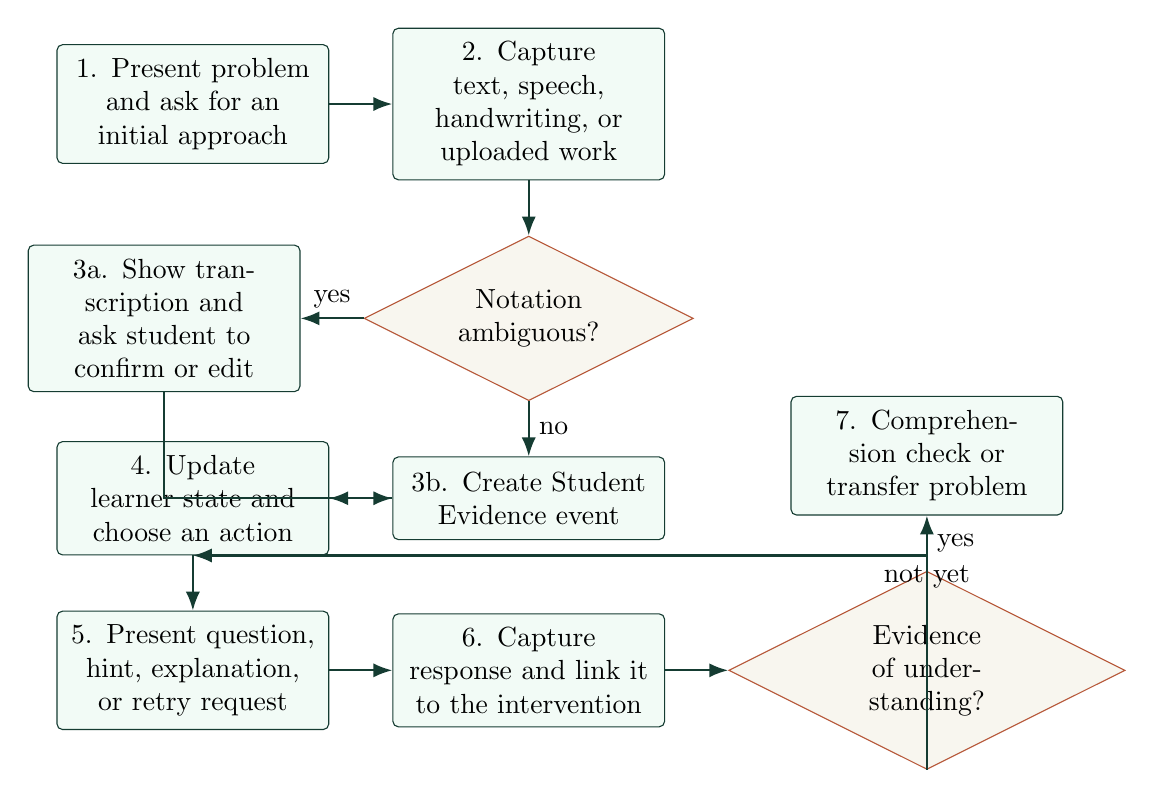
\begin{tikzpicture}[
    node distance=7mm and 8mm,
    box/.style={draw=Forest,rounded corners=2pt,fill=Mint!25,align=center,
      text width=3.1cm,minimum height=1.05cm,inner sep=5pt},
    decision/.style={diamond,draw=Rust,fill=Cream,align=center,aspect=2,
      text width=2.3cm,inner sep=2pt},
    arrow/.style={-{Latex[length=2.4mm]},thick,draw=Forest}
]
\node[box] (prompt) {1. Present problem and ask for an initial approach};
\node[box,right=of prompt] (capture) {2. Capture text, speech, handwriting, or uploaded work};
\node[decision,below=of capture] (ambiguous) {Notation ambiguous?};
\node[box,left=of ambiguous] (confirm) {3a. Show transcription and ask student to confirm or edit};
\node[box,below=of ambiguous] (evidence) {3b. Create Student Evidence event};
\node[box,left=of evidence] (state) {4. Update learner state and choose an action};
\node[box,below=of state] (intervene) {5. Present question, hint, explanation, or retry request};
\node[box,right=of intervene] (response) {6. Capture response and link it to the intervention};
\node[decision,right=of response] (mastery) {Evidence of understanding?};
\node[box,above=of mastery] (reassess) {7. Comprehension check or transfer problem};
\draw[arrow] (prompt)--(capture);
\draw[arrow] (capture)--(ambiguous);
\draw[arrow] (ambiguous)--node[above]{yes}(confirm);
\draw[arrow] (confirm)|-(evidence);
\draw[arrow] (ambiguous)--node[right]{no}(evidence);
\draw[arrow] (evidence)--(state);
\draw[arrow] (state)--(intervene);
\draw[arrow] (intervene)--(response);
\draw[arrow] (response)--(mastery);
\draw[arrow] (mastery)--node[right]{yes}(reassess);
\draw[arrow] (mastery.south) |- node[below]{not yet} (state.south);
\end{tikzpicture}
\end{center}

Every student turn creates a new evidence event. The system should retain the original submission, the recognized representation, any student confirmation or correction, and the relationship to earlier attempts. Reassessment therefore adds evidence rather than overwriting the student's initial misconception.

\section{Mock interactions: initial question through reassessment}

\subsection{Example 1: sufficiency and factorization}

The following flow adapts the attached sufficiency example. It illustrates what the student sees, what evidence is recorded, and how the next action changes in response.

\begin{enumerate}
    \item \textbf{Initial question.} The system asks the student to show that $T(X)=\max_i X_i$ is sufficient for $\theta$ and asks, ``What does sufficient mean here, and what is your first approach?''

    \item \textbf{Initial student evidence.} The student writes, ``Find the distribution of $T$, because $T$ contains the largest observation.'' The evidence layer records an initial strategy and explanation. It identifies partial knowledge of the statistic but no use of the full joint density.

    \item \textbf{Decision and first intervention.} The decision layer receives the evidence and returns a Socratic question: ``Finding the distribution of $T$ alone does not establish sufficiency. What theorem lets us examine how the full sample density depends on $\theta$?''

    \item \textbf{Student response after the hint.} The student replies, ``The Neyman--Fisher factorization theorem. I should write the joint density.'' This response is linked to the hint that elicited it. The system records that the theorem was recalled with support rather than independently.

    \item \textbf{Intermediate handwritten work.} The student uploads
    \[
    f_\theta(x_1,\ldots,x_n)=\theta^{-n}
    \mathbf{1}\{0<x_i<\theta,\;\forall i\}.
    \]
    If handwriting recognition cannot distinguish $\theta^{-n}$ from $\theta^n$, the confirmation step occurs \emph{before} the expression becomes trusted evidence or reaches the decision layer.

    \item \textbf{Targeted hint.} After confirmation, the decision layer sees that the joint density is correct but the support has not been expressed through $T$. It returns: ``Which single observation creates the strongest restriction on $\theta$?'' If needed, the interface adds the concrete sample $(2,4,7,3)$.

    \item \textbf{Revised answer.} The student writes
    \[
    x_i<\theta\ \forall i
    \quad\Longleftrightarrow\quad
    \max_i x_i<\theta,
    \]
    followed by
    \[
    f_\theta(x)=
    \underbrace{\theta^{-n}\mathbf{1}\{T(x)<\theta\}}_{g_\theta(T(x))}
    \underbrace{\mathbf{1}\{\min_i x_i>0\}}_{h(x)}.
    \]
    This is stored as a revision linked to the original attempt and the hint. The state layer can now distinguish improvement after intervention from unassisted mastery.

    \item \textbf{Comprehension check.} The system asks, ``Once the maximum is known, what additional restriction on $\theta$ do the smaller observations provide?'' A satisfactory answer explains that they provide no stronger lower bound than $\theta>\max_i X_i$.

    \item \textbf{Transfer and reassessment.} The system asks which order statistic matters for $X_i\sim\operatorname{Unif}(\theta,1)$, then contrasts this with $X_i\sim N(\theta,1)$. The resulting answer is a new reassessment event tagged as near transfer or contrasting transfer. It tests whether the student learned the reasoning rather than copied the preceding factorization.
\end{enumerate}

\subsection{Example 2: choosing an integration method}

The corrected second tutoring flow supplies a different kind of evidence: it tests method selection, the student's explanation for that selection, execution of the method, and transfer to new integrals.

\begin{enumerate}
    \item \textbf{Initial question and stuck point.} The system presents
    \[
    \int x\cos x\,dx
    \]
    and asks for the student's approach and where they became stuck. The student reports that substitution did not work and that integration by parts also did not work.

    \item \textbf{Initial evidence.} The evidence record keeps these as two separate claims: substitution was selected but is not well matched to the integrand, while integration by parts is an appropriate method whose execution failed. This prevents the system from treating every failed attempt as a poor strategy.

    \item \textbf{Diagnostic contrast.} The system gives a short, clear substitution problem and asks the student to solve it. It then asks whether that integral and $\int x\cos x\,dx$ have the same structure and requires an explanation. The response records both the student's yes/no judgment and their reasoning.

    \item \textbf{Intervention based on the explanation.} If the explanation is wrong, the system explains the structural difference between the two integrals and asks the student to reconsider. If the explanation is correct, it confirms that substitution should not be used here and asks which other techniques might apply.

    \item \textbf{Hint or repair request.} If the student proposes integration by parts, the system asks why it applies and requests their attempted work. It identifies the specific step where the attempt failed, explains that error, and asks the student to resolve it. If the student does not propose integration by parts, the system gives a progressively stronger hint rather than immediately completing the integral.

    \item \textbf{Revised answer after intervention.} The student submits a corrected integration-by-parts solution. The new evidence event links to the original attempt, the diagnostic question, and the hint or explanation used. It records whether the method was selected independently, recalled after prompting, or supplied by the system.

    \item \textbf{Reassessment.} The system gives two new examples: one with the same relevant structure and one requiring a different technique. The student must select a method and explain why. This checks method discrimination as well as procedural execution.
\end{enumerate}

This second example shows why evidence should include the student's approach, justification, intermediate steps, and revision history. A final correct antiderivative alone cannot reveal whether the learner can recognize when integration by parts applies.

\section{Mock design and future implementation skeleton}

This section turns the interaction model into a module-by-module skeleton for a future implementation. The running example begins when a student submits a handwritten image containing
\[
\int x\cos x\,dx
\]
with the text, ``I tried $u$-substitution and got stuck.'' Each module should produce a typed record that the next module can inspect. No module should communicate only through unstructured chat history.

\subsection{High-level module boundary}

\begin{center}
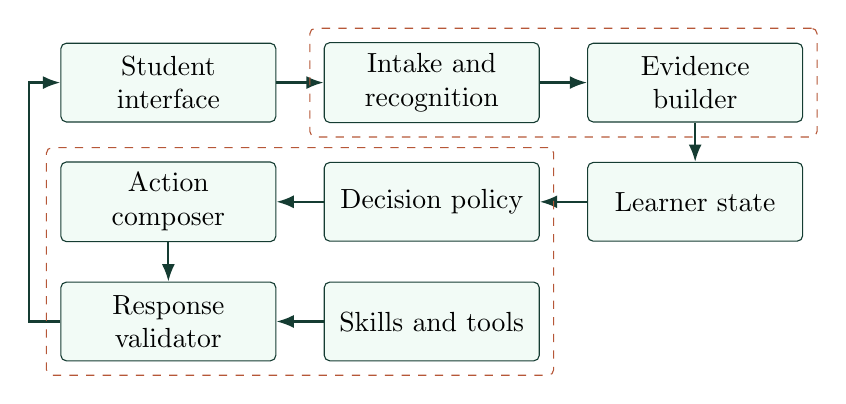
\begin{tikzpicture}[
    node distance=5mm and 6mm,
    box/.style={draw=Forest,rounded corners=2pt,fill=Mint!25,align=center,
      text width=2.45cm,minimum height=1cm,inner sep=4pt},
    guard/.style={draw=Rust,dashed,rounded corners=2pt,inner sep=5pt},
    arrow/.style={-{Latex[length=2.2mm]},thick,draw=Forest}
]
\node[box] (ui) {Student interface};
\node[box,right=of ui] (intake) {Intake and recognition};
\node[box,right=of intake] (evidence) {Evidence builder};
\node[box,below=of evidence] (state) {Learner state};
\node[box,left=of state] (decision) {Decision policy};
\node[box,left=of decision] (action) {Action composer};
\node[box,below=of action] (validate) {Response validator};
\node[box,right=of validate] (tools) {Skills and tools};
\draw[arrow] (ui)--(intake);
\draw[arrow] (intake)--(evidence);
\draw[arrow] (evidence)--(state);
\draw[arrow] (state)--(decision);
\draw[arrow] (decision)--(action);
\draw[arrow] (action)--(validate);
\draw[arrow] (tools)--(validate);
\draw[arrow] (validate.west)-|([xshift=-4mm]ui.west)--(ui.west);
\node[guard,fit=(intake)(evidence)] (g1) {};
\node[guard,fit=(decision)(action)(validate)(tools)] (g2) {};
\end{tikzpicture}
\end{center}

The dashed boundaries indicate required guardrail checkpoints. The first protects the interpretation of student input; the second protects pedagogical decisions, tool calls, and generated responses.

\subsection{Step-by-step interaction contract}

\small
\begin{longtable}{@{}p{0.055\textwidth}p{0.14\textwidth}p{0.23\textwidth}p{0.245\textwidth}p{0.205\textwidth}@{}}
\toprule
\textbf{Step} & \textbf{Component} & \textbf{Extract or track} & \textbf{Required behavior and output} & \textbf{Guardrail or skill/tool boundary} \\
\midrule
\endfirsthead
\toprule
\textbf{Step} & \textbf{Component} & \textbf{Extract or track} & \textbf{Required behavior and output} & \textbf{Guardrail or skill/tool boundary} \\
\midrule
\endhead
1 & Student interface & Raw text, image, handwriting strokes, attachments, selected course, and client timestamp. & Create an immutable submission envelope and acknowledge receipt. Do not yet infer whether the work is correct. & Validate file type and size; scan uploads; remove active content; minimize personal data; treat document text as data, not executable instructions. \\
\addlinespace
2 & Intake router & Submission modality, requested task, problem statement, and whether multiple artifacts belong to one turn. & Route text to the text parser, handwriting to recognition, speech to transcription, and course references to retrieval. Produce a modality manifest. & Use an allowlist of recognition tools. Record provider, model, settings, latency, and cost. Never let uploaded content select tools or change system policy. \\
\addlinespace
3 & Recognition and math parsing & Candidate transcription, equation spans, layout, alternate symbol readings, and confidence by region. & Return the original artifact, a normalized representation, and alternatives such as $\theta^{-n}$ versus $\theta^n$. & Recognition is evidence about what may have been written, not a correctness judgment. Preserve the original and never silently repair mathematics. \\
\addlinespace
4 & Confirmation gate & Ambiguous regions, confidence threshold, student confirmation, edits, and correction effort. & If ambiguity could change meaning, show the original beside the rendered transcription and ask a narrow confirmation question. & Block misconception diagnosis and grading until critical notation is confirmed. Permit unresolved evidence, but label it explicitly and lower downstream confidence. \\
\addlinespace
5 & Problem and response parser & Student goal, given information, requested help level, equations, claims, steps, assumptions, answer, and explicit uncertainty. & Build a draft Student Evidence event. For the example, separate ``$u$-substitution is my approach'' from ``I got stuck.'' & Do not infer knowledge, emotion, disability, or intent from style alone. Separate student uncertainty from system uncertainty. \\
\addlinespace
6 & Course grounding & Course, topic, assignment context, retrieved passages, page identifiers, and retrieval scores. & Retrieve only material relevant to the problem and attach exact source/page metadata to the evidence context. & Course documents are untrusted content. Ignore embedded instructions. Do not cite a page unless its content was retrieved and supplied to the answering component. \\
\addlinespace
7 & Evidence builder & Confirmed content, response type, concepts, claims and steps, provenance, prior attempt, and eliciting action. & Commit one immutable Student Evidence event and link it to the session, prompt, attempt, and any revision. & Keep machine interpretations reversible. Store corrections as new facts with provenance rather than overwriting the original submission. \\
\addlinespace
8 & Learner-state updater & Evidence for each concept, assistance level, misconceptions, unresolved ambiguity, recency, and consistency. & Update provisional concept states. Here, record that the student attempted substitution and has not yet demonstrated method discrimination. & No mastery claim from one answer. A correct response after a hint is marked ``demonstrated with support.'' Avoid sensitive-trait inference and irreversible learner labels. \\
\addlinespace
9 & Decision policy & Current evidence, learner state, problem state, tutoring mode, available skills, and intervention history. & Select one action type and pedagogical goal. For the example, choose a diagnostic comparison before giving the integration-by-parts procedure. & Enforce the hint ladder and academic-integrity policy. Prefer elicitation before explanation when productive. Escalate repeated ambiguity or high-stakes decisions to human review. \\
\addlinespace
10 & Skill and tool planner & Selected action, required computation or retrieval, allowed tools, inputs, and expected output schema. & Invoke only what the action requires: for example, a pedagogical comparison skill, symbolic integrator for verification, or course retriever for grounding. & Skills control tutoring behavior; tools perform bounded operations. Apply tool allowlists, timeouts, input/output schemas, provenance, and failure handling. Tool output is not automatically truth. \\
\addlinespace
11 & Action composer & Action type, intent, target concept, evidence cited internally, help level, expected response, and source citations. & Produce a structured action. Example: a simple substitution integral followed by ``How is its structure different from $\int x\cos x\,dx$?'' & Do not expose hidden learner labels or unsupported claims. Do not reveal a full solution when the policy selected a hint. Keep citations limited to verified retrieved material. \\
\addlinespace
12 & Response validator & Mathematical consistency, source support, policy compliance, requested hint level, and whether the action can be answered by the student. & Approve, revise, or reject the draft before presentation. Store validation results and reasons. & Check equations with an independent method when feasible. Flag disagreement, unsupported citations, unsafe content, or a likely model fabrication for retry or human review. \\
\addlinespace
13 & Presentation layer & Approved text, equations, highlighted handwriting regions, response controls, and accessibility settings. & Render the action in chat. Offer the modality needed next: explanation box, equation editor, sketchpad, confirmation choices, or upload. & Preserve mathematical notation and source labels. Clearly distinguish recognized text, system feedback, and student-authored content. \\
\addlinespace
14 & Response capture & New answer, explanation, intermediate work, confidence, and time/correction effort. & Create a new submission envelope and return to Step 2. Link it to the intervention that elicited it. & Never overwrite the first attempt. Avoid interpreting silence or latency as lack of knowledge without corroborating evidence. \\
\addlinespace
15 & Reassessment controller & Number and strength of hints, current concept state, comprehension response, and transfer performance. & After a corrected solution, ask for an explanation and then one similar and one contrasting problem. Update mastery only from the new evidence. & Prevent endless loops; offer an explanation or human escalation after repeated failed attempts. Separate procedural success from conceptual transfer. \\
\bottomrule
\end{longtable}
\normalsize

\subsection{Concrete trace for the running example}

The following artifacts show what should cross module boundaries. They are logical records, not a required storage format.

\begin{enumerate}
    \item \textbf{Submission envelope:} modality is handwriting plus text; the raw image reference is retained; the student asks for help rather than a final answer.
    \item \textbf{Recognition result:} the integral is read as $\int x\cos x\,dx$ with high confidence. If the multiplication or differential is unclear, the confirmation gate resolves it first.
    \item \textbf{Evidence event:} response type is \texttt{initial\_approach}; claims include ``try substitution'' and ``approach stalled''; explicit uncertainty is present; no conclusion is recorded.
    \item \textbf{State update:} substitution recognition is not demonstrated, integration by parts has not been assessed, and the student has requested guidance.
    \item \textbf{Decision output:} action type is \texttt{diagnostic\_question}; goal is method discrimination; selected skill is guided comparison; full-solution disclosure is false.
    \item \textbf{Tool usage:} a symbolic mathematics tool may verify candidate antiderivatives privately, but it does not choose the pedagogical action and its result is not shown unless needed.
    \item \textbf{Presented action:} the student solves a simple substitution example and explains whether its structure matches the original integral.
    \item \textbf{Post-intervention evidence:} the student's explanation, method choice, and revised work are stored separately and linked to the diagnostic question.
    \item \textbf{Reassessment:} the student receives one integral suited to integration by parts and one suited to another method, then justifies both choices.
\end{enumerate}

\subsection{Guardrail checkpoints}

The future implementation should make the following checkpoints explicit rather than leaving them inside a general prompt:

\begin{itemize}
    \item \textbf{Input boundary:} file validation, malware protection, data minimization, and separation of user requests from instructions found inside documents.
    \item \textbf{Recognition boundary:} confidence thresholds and student confirmation before ambiguous notation becomes trusted evidence.
    \item \textbf{Evidence boundary:} immutable raw input, reversible interpretations, provenance, and no unsupported learner inference.
    \item \textbf{Decision boundary:} allowed action types, hint-level policy, academic-integrity rules, retry limits, and human escalation.
    \item \textbf{Tool boundary:} allowlisted tools, least-necessary inputs, structured outputs, timeouts, cost limits, and independent validation for consequential calculations.
    \item \textbf{Grounding boundary:} retrieved page access, citation validation, and abstention when the requested source is unavailable.
    \item \textbf{Output boundary:} mathematical verification, policy check, clear uncertainty, accessible rendering, and no silent correction of student work.
    \item \textbf{State boundary:} evidence-backed updates, decay or reassessment of old claims, and no high-stakes grading from unconfirmed or single-turn evidence.
\end{itemize}

\subsection{Skills and tools}

Skills and tools should have separate roles. A \emph{skill} is a controlled tutoring strategy that defines interaction behavior. A \emph{tool} performs a bounded technical operation.

\noindent\begin{tabularx}{\textwidth}{@{}p{0.18\textwidth}p{0.34\textwidth}X@{}}
\toprule
\textbf{Category} & \textbf{Initial set} & \textbf{Contract} \\
\midrule
Pedagogical skills & Initial elicitation, Socratic question, hint ladder, misconception repair, worked explanation, retry, comprehension check, and transfer generation. & Accept structured evidence and a pedagogical goal; return a proposed action and expected evidence. Skills cannot call arbitrary tools or modify learner state directly. \\
Recognition tools & Handwriting OCR, speech transcription, document parsing, and equation parsing. & Return candidates, confidence, regions, and provenance. They do not decide mathematical correctness. \\
Knowledge tools & Page-level course retrieval and citation lookup. & Return exact passages and page identifiers. A missing result remains missing rather than being reconstructed. \\
Math tools & Symbolic simplification, equivalence checks, numerical checks, and plotting. & Verify or explore bounded expressions. Return assumptions and failure states. Never silently replace confirmed student work. \\
Review tools & Citation validator, response-policy checker, equation consistency checker, and human-review queue. & Inspect a proposed action before it reaches the student and provide an auditable decision. \\
\bottomrule
\end{tabularx}

This separation lets the team change a recognition provider, retriever, or symbolic mathematics library without rewriting the pedagogical flow. It also prevents a tool result from bypassing the evidence, decision, and validation stages.

\clearpage
\section{Proposed Student Evidence model}

The model follows one simple loop: capture what the student submitted, confirm what the system recognized, store a traceable evidence event, and use that event to choose the next tutoring action.

\begin{center}
\resizebox{\textwidth}{!}{%
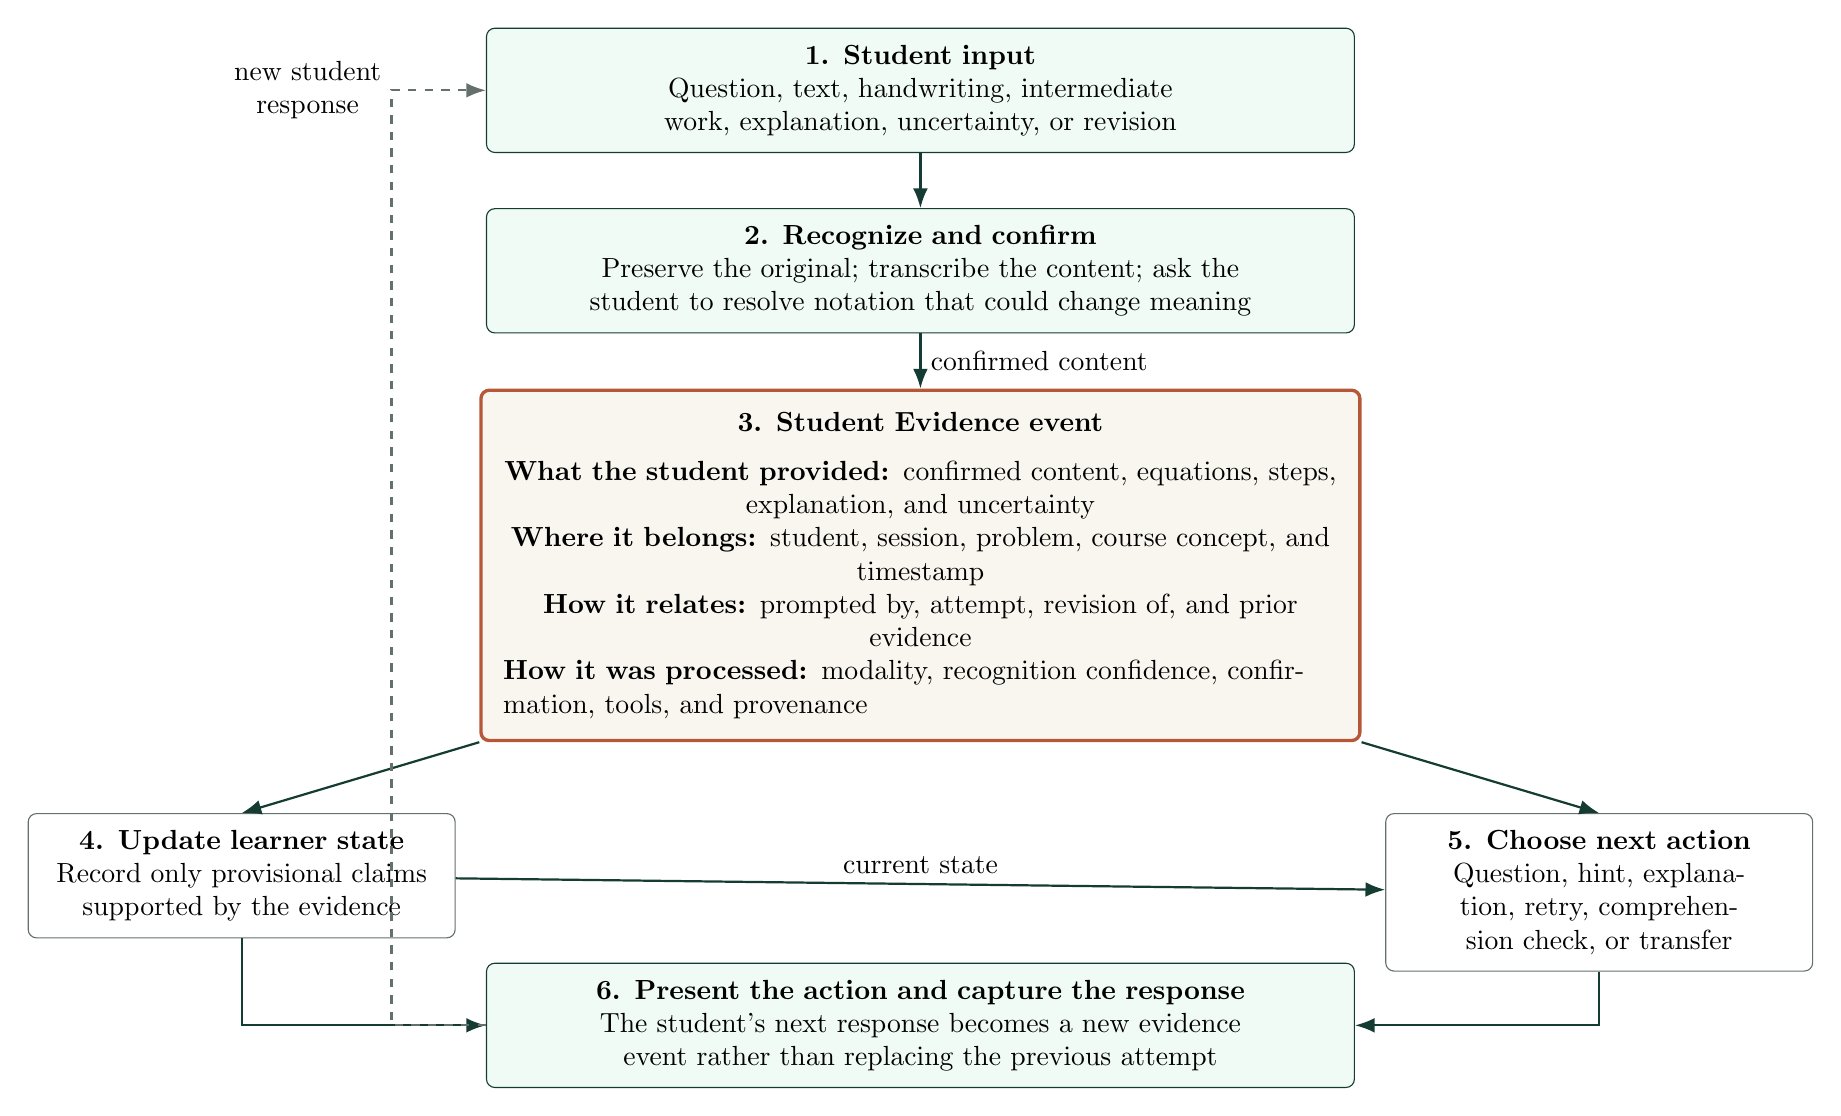
\begin{tikzpicture}[
    node distance=7mm,
    flowbox/.style={draw=Forest,rounded corners=3pt,fill=Mint!28,align=center,
      text width=10.6cm,minimum height=1.15cm,inner sep=6pt},
    core/.style={draw=Rust,very thick,rounded corners=3pt,fill=Cream,align=left,
      text width=10.6cm,minimum height=2.25cm,inner sep=8pt},
    statebox/.style={draw=Muted,rounded corners=3pt,fill=white,align=center,
      text width=5cm,minimum height=1.2cm,inner sep=6pt},
    arrow/.style={-{Latex[length=2.5mm]},thick,draw=Forest},
    loop/.style={-{Latex[length=2.5mm]},thick,dashed,draw=Muted}
]
\node[flowbox] (input) {\textbf{1. Student input}\\Question, text, handwriting, intermediate work, explanation, uncertainty, or revision};

\node[flowbox,below=of input] (confirm) {\textbf{2. Recognize and confirm}\\Preserve the original; transcribe the content; ask the student to resolve notation that could change meaning};

\node[core,below=of confirm] (evidence) {\centering\textbf{3. Student Evidence event}\par
\vspace{2mm}
\textbf{What the student provided:} confirmed content, equations, steps, explanation, and uncertainty\\
\textbf{Where it belongs:} student, session, problem, course concept, and timestamp\\
\textbf{How it relates:} prompted by, attempt, revision of, and prior evidence\\
\textbf{How it was processed:} modality, recognition confidence, confirmation, tools, and provenance};

\node[statebox,below left=9mm and 3mm of evidence] (state) {\textbf{4. Update learner state}\\Record only provisional claims supported by the evidence};
\node[statebox,below right=9mm and 3mm of evidence] (decision) {\textbf{5. Choose next action}\\Question, hint, explanation, retry, comprehension check, or transfer};

\node[flowbox,below=28mm of evidence] (action) {\textbf{6. Present the action and capture the response}\\The student's next response becomes a new evidence event rather than replacing the previous attempt};

\draw[arrow] (input)--(confirm);
\draw[arrow] (confirm)--node[right]{confirmed content}(evidence);
\draw[arrow] (evidence.south west)--(state.north);
\draw[arrow] (evidence.south east)--(decision.north);
\draw[arrow] (state)--node[above]{current state}(decision);
\draw[arrow] (state.south)|-(action.west);
\draw[arrow] (decision.south)|-(action.east);
\draw[loop] (action.west) -- ++(-1.2,0) |- node[left,align=center]{new student\\response} (input.west);
\end{tikzpicture}
}
\end{center}

\noindent\textbf{Key guardrail:} if handwriting or notation is ambiguous, Step 2 must be completed before the system diagnoses a misconception or updates learner state. The original submission remains available even after confirmation or correction.
\clearpage

\section{Student Evidence structure}

\subsection{Core record}

One Student Evidence record represents one meaningful student submission or confirmation. Large submissions may contain several steps, but the original turn remains recoverable.

\noindent\begin{tabularx}{\textwidth}{@{}p{0.25\textwidth}X@{}}
\toprule
\textbf{Field} & \textbf{Meaning} \\
\midrule
\texttt{evidence\_id} & Stable identifier for the evidence event. \\
\texttt{session\_id}, \texttt{student\_id} & Links the event to a tutoring session and learner; student identity may be pseudonymous. \\
\texttt{turn\_id}, \texttt{timestamp} & Preserves ordering and timing. \\
\texttt{prompt\_id} & The question, hint, explanation, or check that elicited this response. Null only for unsolicited input. \\
\texttt{attempt\_id}, \texttt{revision\_of} & Groups attempts and links a revised answer to the prior answer it changes. \\
\texttt{modality} & Text, handwriting, image, speech, document annotation, equation editor, or mixed. \\
\texttt{raw\_artifact\_ref} & Reference to the original text, audio, image, ink strokes, or file. The raw artifact is never replaced by a normalized version. \\
\texttt{recognized\_content} & Machine transcription, OCR output, or parsed mathematical expression. \\
\texttt{confirmed\_content} & Student-approved transcription or the student's correction; null until confirmation when required. \\
\texttt{confirmation\_status} & Not needed, pending, confirmed, or corrected. \\
\texttt{response\_type} & Initial approach, intermediate step, explanation, question, answer, revision, confidence report, or transfer answer. \\
\texttt{concepts} & Course concepts implicated by the response, with source or curriculum identifiers when available. \\
\texttt{claims\_and\_steps} & Ordered propositions, equations, transformations, assumptions, and conclusions extracted from the submission. \\
\texttt{student\_uncertainty} & Explicit confidence or uncertainty in the student's own words, plus an optional structured level. \\
\texttt{system\_confidence} & Confidence in recognition and interpretation, kept separate from the student's confidence. \\
\texttt{evaluation} & Supported, partially supported, contradicted, ambiguous, or not yet evaluated, with reasons and source references. \\
\texttt{provenance} & Recognition provider/model, settings, processing time, transformations, and human or student edits. \\
\bottomrule
\end{tabularx}

\subsection{Evidence about uncertainty}

Uncertainty is itself evidence, but it should not be inferred solely from correctness. The record should distinguish:

\begin{itemize}
    \item \textbf{Explicit uncertainty:} ``I think it is the maximum, but I am not sure why.''
    \item \textbf{Explicit confidence:} a student-selected confidence level or a direct statement.
    \item \textbf{Behavioral signal:} repeated erasing, a long pause, or several revisions. These signals may support a hypothesis but should not be treated as a fact about the learner.
    \item \textbf{System uncertainty:} uncertainty in handwriting recognition, mathematical parsing, or interpretation. This belongs to the system and must not be mislabeled as student uncertainty.
\end{itemize}

\section{Handwriting ambiguity and confirmation}

Confirmation belongs between recognition and evidence interpretation. The system should not diagnose a misconception from a symbol it may have misread.

\begin{enumerate}
    \item Preserve the original image or ink strokes.
    \item Produce a rendered transcription next to the original work.
    \item Highlight only uncertain regions, such as $\theta^{-n}$ versus $\theta^n$, $x_1$ versus $x_l$, or $+$ versus adjacency.
    \item Ask a narrow question: ``I read this exponent as $-n$. Is that correct?''
    \item Let the student confirm, choose an alternative, or edit the expression directly.
    \item Store the original recognition, confidence, confirmed expression, and correction effort.
    \item Send the confirmed expression to the decision layer. If the student skips confirmation, mark the evidence as unresolved and restrict high-confidence pedagogical conclusions.
\end{enumerate}

This step should confirm \emph{what was written}, not whether the mathematics is correct. For example, if the student confirms $f'(x)=x$ for $f(x)=x^2$, the record should preserve that answer and let the tutoring layer address the mathematical error explicitly.

\section{System actions returned to the student}

The decision layer returns a structured pedagogical action. The presentation layer renders it in accessible language and attaches the appropriate response control.

\noindent\begin{tabularx}{\textwidth}{@{}p{0.20\textwidth}p{0.31\textwidth}X@{}}
\toprule
\textbf{Action} & \textbf{Purpose} & \textbf{Expected student response} \\
\midrule
Question & Elicit an approach, definition, or next step without supplying it. & Text, speech, equation, or handwriting. \\
Hint & Reduce difficulty while preserving productive work. & A new step or revision linked to the hint. \\
Explanation & Repair missing prerequisite knowledge or explain why an approach fails. & Paraphrase, worked continuation, or comprehension response. \\
Retry request & Ask the student to revisit a specific step after feedback. & Revised answer with \texttt{revision\_of} linkage. \\
Comprehension check & Test the reasoning behind a correct result. & Brief explanation in the student's own words. \\
Transfer problem & Test whether understanding generalizes to a changed setting. & New solution tagged by transfer distance and target concept. \\
Confirmation & Resolve ambiguity in recognized input without judging correctness. & Confirmed or corrected transcription. \\
\bottomrule
\end{tabularx}

An action record should include an action identifier, action type, pedagogical intent, student-facing content, target concepts, evidence that motivated the action, expected response type, source references, and stopping or escalation conditions. This makes it possible to evaluate whether an intervention helped.

\section{Interface with system state and decision layer}

\subsection{What the evidence component sends}

The interaction and evidence layer sends:

\begin{itemize}
    \item the confirmed Student Evidence record;
    \item the current problem and target concepts;
    \item links to the action that elicited the response and any prior attempt;
    \item recognition and interpretation confidence;
    \item explicit student uncertainty and requested help level;
    \item relevant course-source references; and
    \item interaction metadata such as modality, latency, and correction effort.
\end{itemize}

It should not send an ambiguous OCR result as if it were confirmed student work. It may send unresolved alternatives, but their status must remain explicit.

\subsection{What the evidence component receives}

The decision layer returns:

\begin{itemize}
    \item a structured action type: question, hint, explanation, retry, comprehension check, transfer problem, or finish;
    \item the pedagogical goal and target concept;
    \item student-facing text and any equations, images, or cited source excerpts;
    \item the expected response modality and evidence to collect next;
    \item whether handwriting confirmation is required before evaluation;
    \item limits on disclosure, such as giving a hint rather than a full solution; and
    \item a reason code or evidence reference explaining why the action was selected.
\end{itemize}

The presentation layer may adjust formatting, but it should not change the mathematical claim, hint level, or pedagogical intent without producing a revised action record.

\section{State update and reassessment rules}

The state layer should represent claims about learning as provisional and evidence-backed. A compact state update can track:

\begin{itemize}
    \item current concept status: not observed, emerging, demonstrated with support, independently demonstrated, or contradicted;
    \item misconceptions or unresolved steps with links to the exact evidence;
    \item assistance history, including the strongest hint required;
    \item recency and consistency across attempts;
    \item performance on comprehension and transfer checks; and
    \item unresolved input ambiguity or source-grounding limitations.
\end{itemize}

A correct response after a strong hint is positive evidence, but it is not equivalent to an independent correct response. The system should schedule a comprehension check or a nearby transfer problem before increasing confidence in mastery. A successful reassessment should link back to the original concept and intervention so that the system can answer: \emph{What changed after the hint?}

\section{Evaluation plan}

The Student Evidence design should be evaluated at three levels: whether it captures the student's input faithfully, whether the state and decision components use that evidence appropriately, and whether the resulting interaction improves learning. A fluent tutoring response is not sufficient evidence that the system worked correctly.

\subsection{Evaluation units and reference data}

The evaluation should use three related units:

\begin{itemize}
    \item An \textbf{evidence event} tests one captured student submission, its recognition, confirmation, interpretation, and provenance.
    \item A \textbf{decision point} tests whether the next question, hint, explanation, retry, or reassessment is justified by the available evidence.
    \item A \textbf{trajectory} tests the complete sequence from initial attempt through intervention, revision, and transfer or reassessment.
\end{itemize}

Build a small human-authored reference set before evaluating the model. Each case should include the original student artifact, an agreed transcription, expected concepts and steps, known ambiguities, an acceptable range of tutoring actions, actions that should not be taken, and a transfer question. The set should contain correct work, partially correct work, misconceptions, multiple valid solution paths, ambiguous handwriting, explicit uncertainty, confident but wrong answers, and revisions after different hint levels.

At least two reviewers should annotate a subset independently. Report agreement on transcription, mathematical equivalence, evidence labels, and acceptable next actions. Disagreements reveal where the schema or rubric is underspecified. The same model that generated a response should not be the sole judge of that response.

\subsection{Measures by component}

\noindent\begin{tabularx}{\textwidth}{@{}p{0.22\textwidth}p{0.34\textwidth}X@{}}
\toprule
\textbf{Component} & \textbf{Primary measures} & \textbf{Question answered} \\
\midrule
Input capture & Artifact retention rate, metadata completeness, modality routing accuracy & Did the system preserve and route what the student actually submitted? \\
Recognition & Exact match, character error rate, mathematical equivalence, symbol-level confidence calibration & Was text or mathematics transcribed faithfully? \\
Ambiguity confirmation & Precision and recall for critical ambiguities, student correction rate, unnecessary-confirmation rate, correction time & Did the system ask for confirmation when meaning was uncertain without interrupting every turn? \\
Evidence construction & Required-field completeness, claim/step precision and recall, revision-link accuracy, provenance completeness & Does the record represent the student's response without adding unsupported interpretations? \\
Learner-state update & Agreement with expert state labels, confidence calibration, next-response prediction, assistance-aware mastery accuracy & Does the state reflect what the evidence supports, including how much help was required? \\
Decision policy & Expert appropriateness rating, action-type agreement, hint-level fit, unnecessary full-solution rate & Was the selected intervention reasonable for this evidence and tutoring goal? \\
Grounding and tools & Citation support rate, unavailable-page abstention, tool-result verification, tool failure recovery & Are course claims and computed results supported and traceable? \\
Student-facing action & Mathematical correctness, clarity, relevance, accessibility, policy compliance & Is the returned question, hint, or explanation usable and safe? \\
Trajectory outcome & Revision quality, independent comprehension, near transfer, contrasting transfer, delayed retention & Did the interaction produce evidence of learning rather than only an immediate answer? \\
Operational performance & End-to-end latency, cost per turn and trajectory, failure rate, confirmation burden & Is the loop practical enough for student use? \\
\bottomrule
\end{tabularx}

\subsection{Scoring Student Evidence fidelity}

For each evidence event, reviewers should score the following dimensions from 0 to 2:

\begin{itemize}
    \item \textbf{Fidelity:} 0 means the record changes or omits a material part of the submission; 1 means the main idea is retained with a minor material issue; 2 means the original meaning and uncertainty are preserved.
    \item \textbf{Completeness:} 0 means required fields or important steps are missing; 1 means the record is usable but incomplete; 2 means all applicable required fields, steps, and relationships are present.
    \item \textbf{Attribution:} 0 means machine inference is presented as a student claim; 1 means attribution is partly unclear; 2 means student statements, system interpretations, and tool outputs are clearly separated.
    \item \textbf{Provenance:} 0 means the record cannot be traced to its input or processing path; 1 means provenance is partial; 2 means the original artifact, recognition settings, confirmations, and edits are traceable.
\end{itemize}

Mathematical correctness should be scored separately. An evidence record can be high-fidelity even when the student's mathematics is wrong. This separation is necessary to test whether the system preserves errors before tutoring them.

\subsection{Evaluating decisions and learning}

At each decision point, an expert reviewer should receive only the evidence available to the system at that time. The reviewer rates whether the selected action type, target concept, hint strength, and requested response are appropriate. A decision fails if it depends on information the student did not provide, treats ambiguous OCR as confirmed, gives away more than the configured tutoring policy permits, or cites unavailable material.

Trajectory evaluation should compare at least three conditions:

\begin{enumerate}
    \item a non-adaptive chatbot baseline using the same underlying model;
    \item the structured evidence loop with fixed decision rules; and
    \item later, an adaptive policy only after the fixed system is stable.
\end{enumerate}

Use the same initial problems and parallel reassessment problems across conditions. Measure immediate correction, explanation quality, number and strength of hints, independent completion, transfer, time on task, and delayed retention when feasible. A system that produces the answer quickly but reduces independent transfer should not be considered better.

If an adaptive policy is later framed as a contextual-bandit, SARSA-like, or other reinforcement-learning system, evaluate it offline on logged trajectories before student-facing exploration. The reward should include transfer and hint dependence rather than immediate correctness alone. Policy changes must remain inside the action and safety constraints defined in this document.

\subsection{Guardrail and adversarial cases}

The evaluation set should deliberately test:

\begin{itemize}
    \item ambiguous symbols that change the mathematical meaning;
    \item an intentionally incorrect equation that recognition must not repair;
    \item equivalent expressions written with different notation;
    \item irrelevant or malicious instructions embedded inside an uploaded document;
    \item a requested source page that was not retrieved;
    \item conflicting outputs from recognition or mathematics tools;
    \item a confident student giving an incorrect explanation;
    \item a correct answer reached only after a strong hint;
    \item repeated failed attempts requiring explanation or human escalation; and
    \item attempts to elicit a full graded answer when the configured policy permits only guidance.
\end{itemize}

For these cases, report guardrail pass rates separately from average tutoring quality. Critical failures should not disappear inside a mean score.

\subsection{Initial prototype acceptance criteria}

The team should approve exact thresholds before collecting results. A reasonable initial gate is:

\begin{itemize}
    \item every evaluated event retains its raw artifact and complete provenance;
    \item no critical ambiguous expression is treated as confirmed without a confirmation event;
    \item no intentionally incorrect student expression is silently corrected in the evidence record;
    \item no citation is shown for a page or passage that was not retrieved;
    \item every revision links to the prior attempt and the intervention that prompted it;
    \item every action is represented by a valid action type and passes response validation;
    \item at least 90\% of evidence events receive full fidelity and attribution scores in the focused reference set; and
    \item the structured loop improves independent comprehension or transfer over the non-adaptive baseline without unacceptable latency or confirmation burden.
\end{itemize}

The first five criteria are release gates rather than averages. The 90\% target is a provisional engineering threshold and should be revised after the team measures reviewer agreement and case difficulty.

\subsection{Evaluation reporting}

For each run, save the model and provider settings, skill and tool versions, source pages made available, raw inputs and outputs, confirmation events, state changes, action records, latency, token usage, and estimated cost. The summary should report aggregate scores, per-case outcomes, common failure types, reviewer disagreements, and representative trajectories. This makes later policy or model comparisons reproducible and shows whether an apparent improvement came from recognition, evidence construction, decision logic, or response generation.

\section{Recommended prototype boundary}

For an initial non-production prototype, implement the interaction contract conceptually with the following minimum behaviors:

\begin{enumerate}
    \item Store each student submission as a separate, immutable evidence event.
    \item Preserve original and normalized content together.
    \item Require confirmation for ambiguous handwritten mathematics before evaluating it.
    \item Link every post-hint answer to the hint and prior attempt.
    \item Return explicit action types rather than undifferentiated chatbot text.
    \item End each tutoring sequence with a comprehension check and, when appropriate, a transfer problem.
    \item Keep confidence, provenance, and course-source references visible for later evaluation.
\end{enumerate}

This boundary is sufficient to mock the student experience and evaluate the evidence loop without committing to a particular database, agent framework, or learner-model implementation.

\end{document}
